\documentclass{article}
\usepackage[top=1in,right=1in,bottom=1in,left=1in]{geometry}
\usepackage[utf8]{inputenc}
\usepackage{titlesec}
\usepackage{amsmath}
\usepackage{amssymb}
\usepackage{graphicx}
\usepackage{float}
\usepackage{parskip}
\usepackage{url}
\usepackage{syntax}
\usepackage{xspace}
\usepackage{multicol}
\usepackage{algorithm}
\usepackage[noend]{algpseudocode}
\usepackage{todonotes}

\usepackage{color}
  \definecolor{dkblue}{rgb}{0,0.1,0.5}
  \definecolor{lightblue}{rgb}{0,0.5,0.5}
  \definecolor{dkgreen}{rgb}{0,0.4,0}
  \definecolor{dk2green}{rgb}{0.4,0,0}
  \definecolor{dkviolet}{rgb}{0.6,0,0.8}
  \definecolor{dkpink}{rgb}{0.2,0,0.6}
\usepackage{listings}
  \def\lstlanguagefiles{coq-listing.tex}
\lstset{language=SSR}
\lstset{frame=single}
\lstset{moredelim=[is][]{|*}{*|}}
\lstset{moredelim=*[is][\itshape\rmfamily]{/*}{*/}}

\renewcommand{\todo}[1]{{\color{red}\textbf{[TODO: #1]}}}

% Language
\newcommand{\imp}{\textsc{Imp}\xspace}
\newcommand{\comskip}{\texttt{skip}\xspace}
\newcommand{\comgc}{\texttt{GC}\xspace}
\newcommand{\comif}[3]{\texttt{if}\ #1\  \texttt{then}\ \{#2\}\ \texttt{else}\ \{#3\}\xspace}
\newcommand{\comprint}[1]{\texttt{print}\ #1\xspace}
\newcommand{\comseq}[2]{#1;\ #1\xspace}

\newcommand{\booltrue}{\texttt{true}}
\newcommand{\boolfalse}{\texttt{false}}


\title{Verified Garbage Collection: Report}
\author{Alex Renda (adr74), Matthew Li (ml927)}
\date{\today}

\begin{document}
\maketitle
%\begin{multicols*}{2}
\section{Introduction}
In this project, we implement a garbage collector and attempt to prove it correct. Specifically, we implement a mark-sweep collector, which is designed in such a way that it can be easily extended to mark-sweep-compact pending future work.

Mark-sweep GC works in two phases. During the mark phase, the GC traverses the heap and marks all reachable objects. Next, in the sweep phase the GC removes any unmarked objects from the heap. Mark-sweep is a ``halt the world'' GC, so it is always run atomically. We give no explicit control over the GC, and as such it can be run at any time during program execution, between any other two commands.

We chose to mark-sweep since it is a relatively simple, synchronous GC algorithm, so we do not need to model asynchrony of any sort. Additionally, it easily extends to mark-sweep-compact, which we considered a good extension as an extra challenge. As such, mark-sweep seemed to be perfect decision for an initial GC algorithm to prove correct.

At a high level our project consists of
\begin{itemize}
    \item A heap representation
    \item A language and corresponding interpreter for manipulating the heap
    \item A mark-sweep garbage collection implementation (shallow embedding)
    \item A proof that our GC is capable of removing unreachable garbage from our heap (liveness)
    \item A proof that our GC does not remove ``non-garbage" from our heap (safety)
    \item A proof that our GC does not impact the output of a program (correctness). At the time of submission, this proof is still in progress.
\end{itemize}

\section{Heap}
\subsection{Design}
\subsubsection{Abstract representation}
Abstractly, our heap is composed of a graph of heterogenous collections of pointers and integers, paired with a set of marked ``root'' pointers. Our fundamental datatype is a \texttt{val}, which is a sum type of a pointer and an integer. (Unlike some other heap-based languages, integers and pointers are entirely disjoint in our language. This could be implemented in a real system just by tagging a bit of each memory value with ``integer'' or ``pointer''). Each element in the heap is a fixed-length list of \texttt{val}s, where the length is set at allocation time. Our heap has no invariants about dangling pointers --- these just do not create any edges in the heap graph.

\begin{figure}[H]
    \centering
    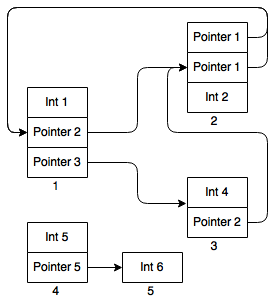
\includegraphics[width=0.4\textwidth]{report/images/heapBasic}
    \caption{A basic heap. The values below each block are the memory location of that block.}
    \label{fig:basic-heap}
\end{figure}

\subsubsection{Physical representation}
Our heap is physically represented as an association list of type:
\mbox{\lstinline|list (ptr_t * struct_t)|}. For instance, the heap in Figure~\ref{fig:basic-heap} could be represented by:

\begin{lstlisting}
[ (4, [Int 5; Pointer 5]) ; (3, [Int 4; Pointer 2]) ; (1, [Int 1; Pointer 2; Pointer 3]) ; (5, [Int 6]) ; (2, [Pointer 1; Pointer 1; Int 2]) ]
\end{lstlisting}

We do assert the physical invariant that there are no duplicate keys in the entire association list. While this kills efficiency, it allows for much easier implementations and proofs, since it much more closely represents the actual invariants that graphs have. Our proofs, conceptually at least, also do not rely on this physical implementation. Any induction over the heap is identical to an induction over nodes in a graph, and could be replaced by that equivalent on any other physical representation of the heap.

\subsubsection{Ideal representation}
If we were start the project from scratch, this choice of physical representation would be the first thing that we would change. Not only are we effectively using a map to represent a graph, which has many of its own issues (some of our proofs by induction on the elements of the heap would have been much more natural to do as induction over the edges of a graph), but we're using a list to represent that map without adequate library support for the abstraction. By the time we were in the thick of proving things, we found that dealing with this heap representation took a large chunk of our time, when the majority of the properties we needed from it should have been free.

\subsection{Reachability}
Our proofs about garbage collection center around a concept of ``reachability'': whether there is some traversal of the heap from a root node that ends at any given struct.
We codified this via an inductive predicate \lstinline|addresses| over pointers and heaps.
A heap and an initial pointer \textit{address} a destination pointer iff there exists a list of indices into structs along the path (conceptually, a list of the turns to take while following the heap graph) that goes from the source pointer to the destination pointer (see Figure \ref{fig:address}).
The full set of reachable objects is then the union of every reachable pointer from every pointer in the root set.

Surprisingly difficult was proving the correspondence between our concept of ``reachability'', and actual reachability through the constructs that are available in the defined language.
It would be possible, for instance, to define a language (like C) that allows for creation of arbitrary pointers, and therefore arbitrary reachability.
We were careful to restrict our language to only be able to access pointers through the \texttt{New} command and dereferencing, which means that the language's definition of reachability is a subset of (and likely equal to) ours.

\begin{figure*}
    \centering
    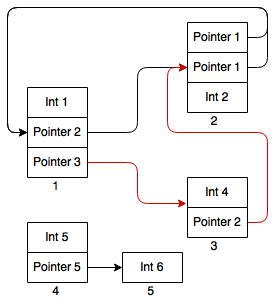
\includegraphics[width=0.4\textwidth]{images/heapAddresses}
    \caption{[2 ; 2] addresses pointer $p=2$ from initial pointer $p=1$. $p=4$ is not addressable from $p=1$.}
    \label{fig:address}
\end{figure*}

\section{Garbage Collection}

A majority of our effort with the project was spent on proving what we call the \lstinline|pointer_equivalence| lemma, which states that anything reachable from the root pointers before garbage collection \emph{must} be reachable from the pointers via the \emph{same path} after garbage collection.

Our approach to this fell along the two natural steps in a mark-sweep garbage collector: we first mark the entire set of reachable pointers, then removed every unreachable pointer from the heap in a sweep step. Compact, if we had gotten to it, would have involved renaming the set of remaining pointers to the most compact set (i.e. the smallest integer value for each pointers).

\subsection{Mark Algorithm}
Within mark-sweep, and the project overall, mark was by far the highest proof effort. This was mainly due to a bad first implementation, which took us several days to attempt proofs on. Once we gave up on the bad implementation and switched to a more tractable one, the overall proofs fell out within about a day. In this section, we discuss each of our attempts, and why we believe our second implementation was easier to work with.


\begin{figure}[H]
\begin{minipage}{0.49\textwidth}
\begin{algorithm}[H]
   \caption{Depth-first Search}
   \label{alg:dfs}
\begin{algorithmic}[0]
  \State {\bfseries Require:} $fuel$: maximum recursion depth
  \State {\bfseries Require:} $roots$: set of root pointers
  
    \Function{Mark Pointer}{$fuel, p$}
     \If {$fuel = 0$}
     \Return $\{p\}$
     \EndIf
     \State $ps \leftarrow \bigcup_{(p, p') \in E}$ \Call{Mark Pointer}{$fuel - 1, p'$}
     \State
     \Return $\{p\} \cup ps$ 
     
    \EndFunction
    \State
    \Return $\bigcup_{p \in roots}$ \Call{Mark Pointer}{$|E|, p$}
\end{algorithmic}
\end{algorithm}
\end{minipage}
\begin{minipage}{0.49\textwidth}
\begin{algorithm}[H]
   \caption{Fixpoint}
   \label{alg:fixpoint}
\begin{algorithmic}[0]
  \State {\bfseries Initialize:} $p_{new}$: set of initial (root) pointers
 \Repeat 
 \State $p_{old} \leftarrow p_{new}$
 \State $p_{step} \leftarrow \{p\ |\ \exists p' \in p_{old}, (p', p) \in E\}$
 \State $p_{new} \leftarrow p_{old} \cup p_{step}$
 \Until{$|p_{old}| = |p_{new}|$}
 \State
 \Return $p_{new}$
\end{algorithmic}
\end{algorithm}
\end{minipage}
\end{figure}

\paragraph{DFS Algorithm}
Our first attempt at the garbage collection algorithm came from a pure implementation perspective, and likely failed for that same reason.

We first implemented garbage collection as a depth-first through over the heap, dealing with the potential cyclic nature by giving the search a finite amount of fuel, initially the length of the heap (as any reachable pointer can be reached in a path of at most the length of the heap).
This approach is described in Algorithm~\ref{alg:dfs}.

We were actually able to prove most properties about marking all reachable pointers about this algorithm, but we were entirely stuck on the argument that the amount of fuel we gave was sufficient. 
Specifically, we found that in some sense, \emph{too much} was changing in each recursive call: we generally found that any inductive definition we wrote was not strong enough for a DFS that moves around the heap graph.
Ultimately, with this algorithm we were unable to prove the property stated above, that any reachable pointer can be reached in a path of at most the length of the heap.
While intuitively true, we found that arguing this about \textit{paths} was tricky, since this proof would involve splicing together paths around points found in a cycle.

Instead, after significant effort, we gave up on this approach, opting for what we call the Fixpoint Algorithm.

\paragraph{Fixpoint Algorithm}
Many of the issues we had in the first algorithm can be succinctly described as it not behaving nicely when we try to find its fixed point; i.e. that it's hard to prove that it's a monotonically increasing function that saturates after a certain point. To correctly represent that, we chose the less obvious approach shown in Algorithm~\ref{alg:fixpoint}.

This approach, which is effectively a breadth-first search as opposed to a depth-first search, is much more explicit about the fixed point properties of the algorithm: we continue running each pass of the breadth-first search until we find no new points, at which point we can be confident that the algorithm has saturated. Since we're only unioning, we can also be confident that our algorithm is monotonically increasing.

We ultimately found it much easier to conduct all of our proofs with this second approach, as induction (\lstinline|functional induction| specifically) was very easily able to let us make an argument about each case of the algorithm: that either we are taking a single step in a breadth first search, or that there are no more steps to be taken since we reach no new pointers. This approach lets us not have to reason about cycles at all, and was overall a much better fit for the proof style supported by Coq.


\subsection{Safety}
Safety is the first major property we attempted to prove. We define safety using our definition of reachability and the property has three portions:
\begin{itemize}
    \item The GC algorithm does not delete anything reachable from the heap.
    \item The GC algorithm does not add anything reachable to the heap.
    \item The GC algorithm does not change the output of the current state.
\end{itemize}

Proving that the GC algorithm does not change output is trivial, since GC does not change output at all.

Proving that the GC algorithm does not delete anything reachable is the majority of our work on this project. The general overview is that we first show that mark is powerful enough to mark all reachable pointers, which forms the vast majority of the proof effort on this project and is what required us to rewrite our mark algorithm. Afterwards, we simply show that sweep does not remove any of these pointers, and with a few more intermediate lemmas we are able to show that we do not delete anything reachable from the heap. The two most important intermediary lemmas are \lstinline|pointer_equivalence| and \lstinline|value_equivalence|, which we will talk more about below in the implementation section.

Proving that the GC algorithm does not add anything reachable is easier than the other direction, since we do not need to reason about mark at all. Our proof consists of an argument that any struct still present after sweep must have been there before sweep, followed by an argument that this is true for each reachable address. 

\subsection{Liveness}
Liveness is the corresponding property to safety. The goal would be to state that ``after GC, there is no more garbage in the heap". We define garbage as values in the heap that are not reachable. Therefore, what we prove is that after GC, everything in the heap must be reachable.

To do this, we first show that everything we mark must be reachable. While this sounds relatively easy, this actually turned out to be a lot of proof effort and required rewriting aspects of the mark algorithm multiple times. Afterwards, we show that everything left in the heap after sweep must have been marked. From there, it is relatively easy to show that everything remaining in the heap must be reachable. Like safety, \lstinline|pointer_equivalence| is a key lemma for this proof.

\section{Language}
To show that our garbage collection is actually useful, we also implemented a language that could use the heap, and are in the progress of proving that running an atomic stop-the-world garbage collection step between any commands does not affect the result of the program. Specifically, we will show that all traces of program execution (i.e. all sequences of output) remain the same with and without garbage collection. This property is only shown for programs that correctly execute in the first place --- it is likely true for all programs, but we consider the crash case to be relatively uninteresting.

As stated, our proof for this part is still incomplete. We believe it to be true, and to not require significant restructing, but there are a couple of nontrivial lemmas left to be proved before this is complete. We estimate the remaining work will take roughly 1 person-day.

\subsection{Language definition}
\begin{figure}[H]
    \centering
\begin{lstlisting}
Inductive valexp :=
| IntExp : nat -> valexp       (* n *)
| Deref : var -> nat -> valexp (* v[n] *)

Inductive com :=
| New : var -> list valexp -> com         (* var = malloc(length l) ; var[:] = l *)
| AssignMem : var -> nat -> valexp -> com (* var[i] = val *)
| AssignVar : var -> valexp -> com        (* assert(type(val) = Ptr) : var = val *)
| Drop : var -> com                       (* del var *)
| Out : valexp -> com                     (* assert(type(val) = Int) ; print(val) *)
\end{lstlisting}
    \caption{Language definition}
    \label{fig:language}
\end{figure}

Our language is shown in Figure~\ref{fig:language}. 
Essentially, the language maintains a set of local root variables (\lstinline|var|s), and can create and modify elements in the heap via \lstinline|New| and \lstinline|AssignMem| respectively.
A program is a stream of those instructions. While relatively simple, there are a few important design decisions of our language:

\begin{itemize}
\item There is no way to print out or take action based on the \emph{value} of a pointer. This is to enable a potential future compact, which could change pointer values
\item There must be a way to create garbage that the garbage collector can deal with in order for our proofs to be interesting. We actually have two ways to do this in our language, \lstinline|AssignVar| and \lstinline|Drop|, which both overwrite the value of a pointer variable
\item Programs can crash, via dereferencing a variable that does not exist, or indexing too far into a struct. We make no claims or guarantees about this, other than our later proof that GC induces no \emph{new} crashes
\end{itemize}

\subsection{Correctness}
Our correctness property relies on an abstraction shown in Figure~\ref{fig:equiv}: equivalency classes of heaps. Essentially, we define an equivalence relation over heaps (really, over states which are the heap + roots + output so far), which states that between two equivalent states, any path to an \emph{Int} from a root must be identical between both.

We then used this equivalency class to make two arguments. First, garbage collection produces another state in the same equivalency class. Second, given a command and a starting equivalency class of states, you will always end up in a second equivalency class.

With this property about equivalency classes stated, it was relatively easy to show that GC does not change the trace of a program, since it has no effect on the path of equivalent states that a program goes through.

\begin{figure}[H]
    \centering
    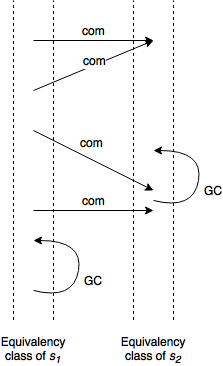
\includegraphics[height=0.4\textheight]{images/equiv}
    \caption{Stepping among equivalency classes}
    \label{fig:equiv}
\end{figure}

\section{Implementation}
In our implementation, we broke down our project into 6 primary files
\begin{itemize}
    \item \textbf{Language.v} This is our language and heap definitions and useful proofs about how our heap works.
    \item \textbf{Gc.v} This is our largest file and includes both our actual GC algorithm (mark-sweep) as well as many useful proofs about our GC algorithm that liveness and safety both depend on.
    \item \textbf{Liveness.v} This file proves the liveness property.
    \item \textbf{Safety.v} This file proves the safety property.
    \item \textbf{Correctness.v} This file proves the correctness property.
    \item \textbf{Util.v} This file contains some useful lemmas about lists and sets that aren't provided by coq but are useful for proving things in our other files.
\end{itemize}

Ultimately, one should consider Liveness and Correctness as our two top level files. These contain the final properties we were attempting to prove (GC removes garbage and GC does not change output). Safety is the critical property that allows correctness to proven.

\subsection{Language.v}
Language contains mostly the definition of our language and heap. We have shown our language definition previously, and the heap is just an association list from pointers to a struct of values. We also define roots, which are an association list from variables to pointers. We define all our values this way (especially the heap mappoing pointers to a struct) so that it easier to prove things about our language. If we were to redo our project, we likely would have changed our model of our heap and roots, as stated earlier.

Also included in this file is our interpreter for a list of commands in our language. This interpreter works by defining the small step semantics. We use this interpreter in our proof of correctness.

The rest of the file is various proofs about our heap and roots that frequently come up. Most of these proofs are necessary since they are association lists, which is why we would have preferred to model both differently.

\subsection{Gc.v}
The main thing this file contains is our GC function, which takes in a state and output a new state after running garbage collection on it.

\begin{lstlisting}
Definition gc (s : state) : state :=
  let roots := (roots s) in
  let heap := (heap s) in
  let output := (output s) in
  let (roots', heap') := compact roots (mark_sweep roots heap) in
  mkState roots' heap' output.
\end{lstlisting}

One thing to note is that we do actually support compact in our GC function and most of our proofs would allow it. However, right now compact is simply a NOP that returns the roots and heap that was input in. This is because two critical proofs in this file do not support compact: \lstinline|pointer_equivalence| and \lstinline|value_equivalence|.

\begin{lstlisting}
Lemma pointer_equivalence :
  forall address r h v p p',
    roots_maps r v p ->
    addresses h p address p' ->
    addresses (mark_sweep r h) p address p'.

Lemma value_equivalence :
  forall r h h' p vs vs',
    (mark_sweep r h) = h' ->
    heap_maps_struct h p vs ->
    heap_maps_struct h' p vs' ->
    vs = vs'.
\end{lstlisting}

Clearly these lemmas don't hold once compact is added (pointers are changed, which also means values would have to be changed). Unfortunately, both are critical for proving safety and liveness, so we would need to prove new lemmas about compact.

This file is also by far where the most proof effort was spent. Specifically the \lstinline|mark_ptrs| function is the bane of our existence, as mentioned above. The mass majority of this file is devoted to proving lemmas about it.

\subsection{Safety.v}
Safety is focused on proving the \lstinline|gc_safety| theorem below:

\begin{lstlisting}
(* All integers reachable using the same variable, address, and index. *)
Definition equiv' (s1 s2: state) : Prop :=
  forall v p1 address p1' k i,
      roots_maps (roots s1) v p1 ->
      addresses (heap s1) p1 address p1' ->
      heap_maps (heap s1) p1' k (Int i) ->
      exists p2 p2',
        roots_maps (roots s2) v p2 /\
        addresses (heap s2) p2 address p2' /\
        heap_maps (heap s2) p2' k (Int i).

(* States are equal if they are equiv' in both directions and have the same output *)
Definition equiv (s1 s2: state) : Prop :=
  (output s1 = output s2) /\ equiv' s1 s2 /\ equiv' s2 s1.

(* State before and GC are equivalent *)
Theorem gc_safety :
  forall st, equiv st (gc st).
\end{lstlisting}

The general idea is we define a concept of equivalence between two states, which matches up with our description of safety from before. One thing to note is that equivalence does require \lstinline|equiv'| holds in both directions (post-GC state to pre-GC state and vice versa). This leads to one of our few admitted proofs:

\begin{lstlisting}
Theorem gc_backward_safety :
  forall st, equiv' (gc st) st
.
Proof.
Admitted.
\end{lstlisting}

We realized late in the project that we needed to show that all integers that are reachable in the post-GC state are reachable in the pre-GC state. This is slightly different from liveness, since there is nothing to say we did not add new roots or new address paths through the heap during GC. Since we only focused on proving the forward relationship, we did not have the time to restructure all our proofs to allow for proving the backward relationship too.

\subsection{Liveness.v}
Liveness is focused on proving the \lstinline|gc_liveness| theorem below:

\begin{lstlisting}
Theorem gc_liveness :
  forall st st' p vs h,
    gc st = st' ->
    (heap st') = h ->
    heap_maps_struct h p vs ->
    exists address v p',
      roots_maps (roots st') v p'
      /\
      addresses h p' address p.
\end{lstlisting}

Recall that this theorem says that after GC, everything in the heap can be reached by an address. Liveness is completely proven for the mark-sweep, there are no admits.

\subsection{Correctness.v}
Correctness is focused on proving the two theorems below, which form our correctness property:

\begin{lstlisting}
Theorem execution_output_exists :
  forall coms st st' out,
    execution st coms out ->
    equiv st st' ->
    exists out',
      execution st' coms out'.

Theorem execution_output_equiv :
  forall coms st st' out out',
    execution st coms out ->
    execution st' coms out' ->
    equiv st st' ->
    out = out'.
\end{lstlisting}

The first theorem states that for every execution of a list of commands, switching the state for an equivalent state still produces an output. The second theorem then extends this to say that the output produced from two equivalent states is identical. Since safety is a proof that GC produces an equivalent state, this is sufficient to show that GC does not change our output which is our correctness property.

\subsection{Util.v}
Utilities consists of a bunch of random and small lemmas that are useful for our proofs. They are generally about coq lists or sets. An example of a particularly useful lemma is below:

\begin{lstlisting}
Lemma in_split_l_ht :
  forall {A B: Type} (l: list (A * B)) p a b (eq_dec: forall n m : A, {n = m} + {n <> m}),
    In p (fst (split l)) \/ p = a <->
    In p (fst (split ((a, b) :: l))).
\end{lstlisting}

This lemma allows us to deal with using cons and split together, which becomes critical whenever we are trying to do induction on our heap. Most of the file consists of lemmas like this one.

\section{Future Work}
As stated above, there is a lot of future work for us to do on this project. Our highest priority would be to complete our proofs, including the admitted lemmas. The most impotent lemma is \lstinline|gc_backward_safety|, which will likely require us to prove a whole new set of properties about our GC algorithm.

Another large extension that we mostly support is changing our algorithm to mark-sweep-compact instead of just mark-sweep. As stated before, this is mostly supported since we designed our proofs with compact in mind. We would need to extend \lstinline|pointer_equivalence| and \lstinline|value_equivalence| (since those don't hold for compact). This likely requires figuring out a key lemma about compact so that safety and liveness still hold. Afterwards, all the other proofs should stay the same.

\section{Conclusion}
Overall, this project took us $\frac{1}{3}$ person years (py). The primary effort was spent on the Gc.v file as stated above, we estimate roughly $\frac{1}{6}$ py. Specifically, the majority of our time was spent on rewriting and reproving mark. Many times, proving one version of mark to support one proof would make another proof extremely difficult.

We had hoped to prove compact and also submit a project with no admits. Unfortunately, that clearly did not happen. While we don't think any of the admits we have are particularly difficult or impossible to prove theorems, we didn't end up having the time to prove them. Additionally, we put a lot of effort earlier on into supporting compact but in the end our liveness and safety proofs rely on compact being unimplemented.

Our primary take away from this project is that proving even a relatively simple algorithm is a lot of work in Coq. A lot of this work is caused by the algorithms and representation themselves. The amount of times we had to rewrite our algorithm is a testament to that. If given the opportunity we would definitely setup \texttt{Language.v} very differently. For instance, many of the proofs would have been a lot easier had the heap actually been modeled as a graph.

Another takeaway is that we definitely should have started with the higher level theorems we needed to prove earlier. We didn't realize we needed to prove \lstinline|gc_backward_safety| until far too late (about 12 hours before the assignment was due), but if we had started with our correctness proof earlier we would have realized this.

Overall, we are happy with our project and what we were able to prove. We really enjoyed this class!
%\end{multicols*}
\end{document}